\subsection{Timing Performance Results from Calorimeter with SiPM Readout}
\label{sec:beamtiming}

Four different SiPMs are used to read out the four light fibers. Data are taken with electron
beam energy at $20$, $50$, $100$, $150$, and $200$~GeV, and the time resolution
measured for each beam energy is plotted as a function of the mean signal
amplitude measured in the same dataset in Figure~\ref{TimeResolution}. We show
the time resolution of the four individual fibers separately as a function of their
respective mean signal amplitudes for both the DSB-doped fibers and the DSB-filled
quartz capillaries. The mean signal amplitude increases as the beam energy 
increases. We observe that the time resolution improves as the 
signal amplitude (or beam energy) increases. The best time resolution per fiber is around
$60$~ps for all of the channels, but the amplitude at which this performance is
achieved varies. 

The variation of signal amplitudes is due to variations in the operational gain
of the four SiPMs. As discussed in Section~\ref{sec:LYSOSiPMSetup}, each SiPM
was operated at a bias voltage of $70$~V. As the breakdown voltages for each
SiPM varies slightly, the over-voltages also vary resulting in significant
differences in gain. Furthermore, the SiPM-to-fiber coupling may not be perfectly
identical, resulting in a small variation of light collection efficiency. The combination of these effects
explains why the best time resolutions are achieved at different signal amplitudes in the four
different channels.

Another important observation is that the time resolution
measured from the WLS fibers fall on the same curve as the time
resolution measured from the quartz capillaries. We conclude that the method of
light extraction impacts the time resolution only through its effect on the
signal amplitude, and no additional time jitter is introduced. 


\begin{figure}[!htb]
\centering
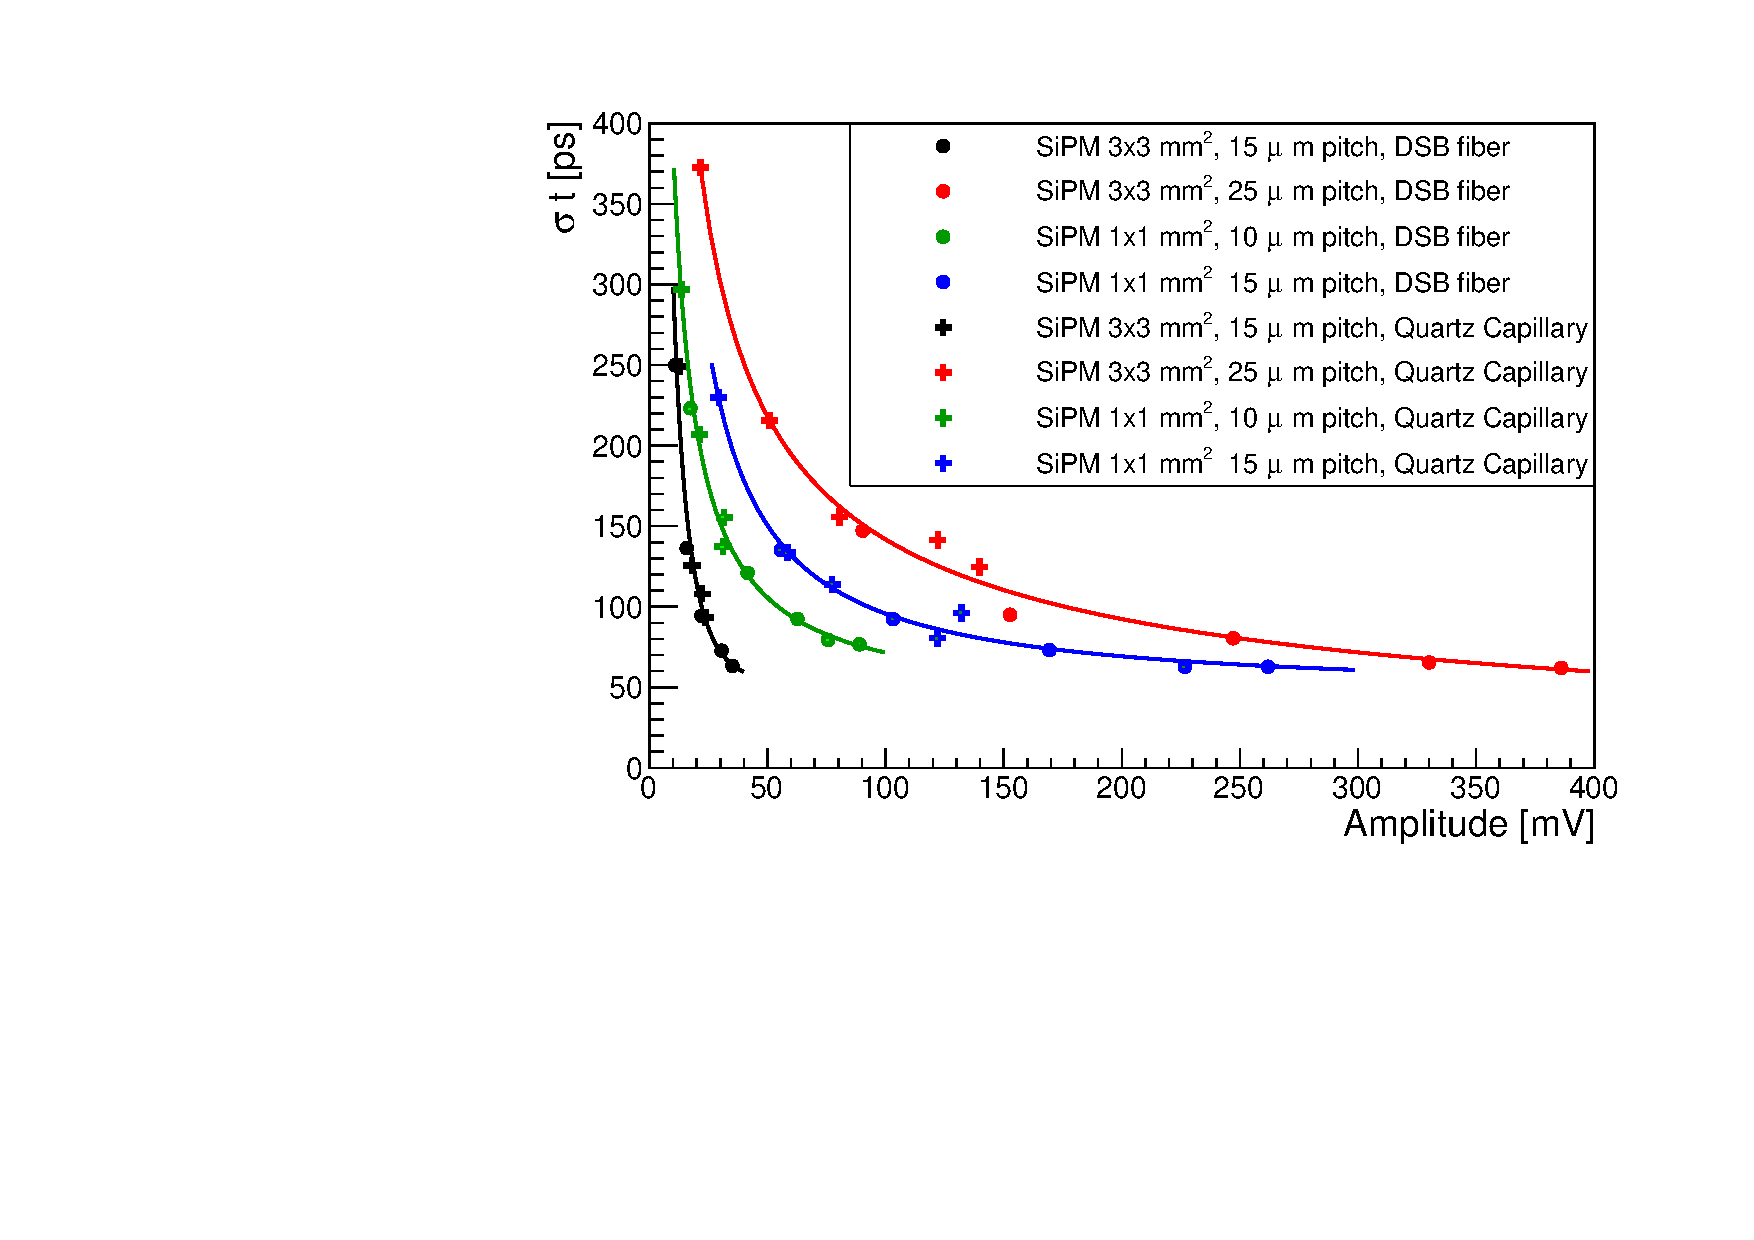
\includegraphics[width=0.99\textwidth]{figures/ShashlikTimeResolution.pdf}
\caption{\label{TimeResolution} The measured time resolution is shown as a
function of the signal amplitude for each individual read-out fiber and SiPM.
The data for each SiPM consists of two sets, one with the DSB-doped WLS plastic fiber
shown as dots and one with the capillaries filled with a liquid DSB-based WLS shown as
squares. }
\end{figure}


As the time measurement precision depends on the rise time of the pulse we also
measure the time resolution as a function of the rise time for signals observed
in the calorimeter cell shown in Figure~\ref{RiseTime}. As in
Figure~\ref{TimeResolution}, the data points correspond to measurements of the
time resolution and mean rise time for datasets collected using electron beam
energies ranging from $20$~GeV to $200$~GeV. The capacitance of the high-pass
filter for the $3\times3$~$\mathrm{mm}^{2}$ SiPM with $25$~$\mu$m pixel size is
$100$~pF, which is significantly larger than the capacitance for the other three
SiPMs ($15$~pF), resulting in signals with larger amplitude but also larger rise
time.

\begin{figure}[!htb]
\centering
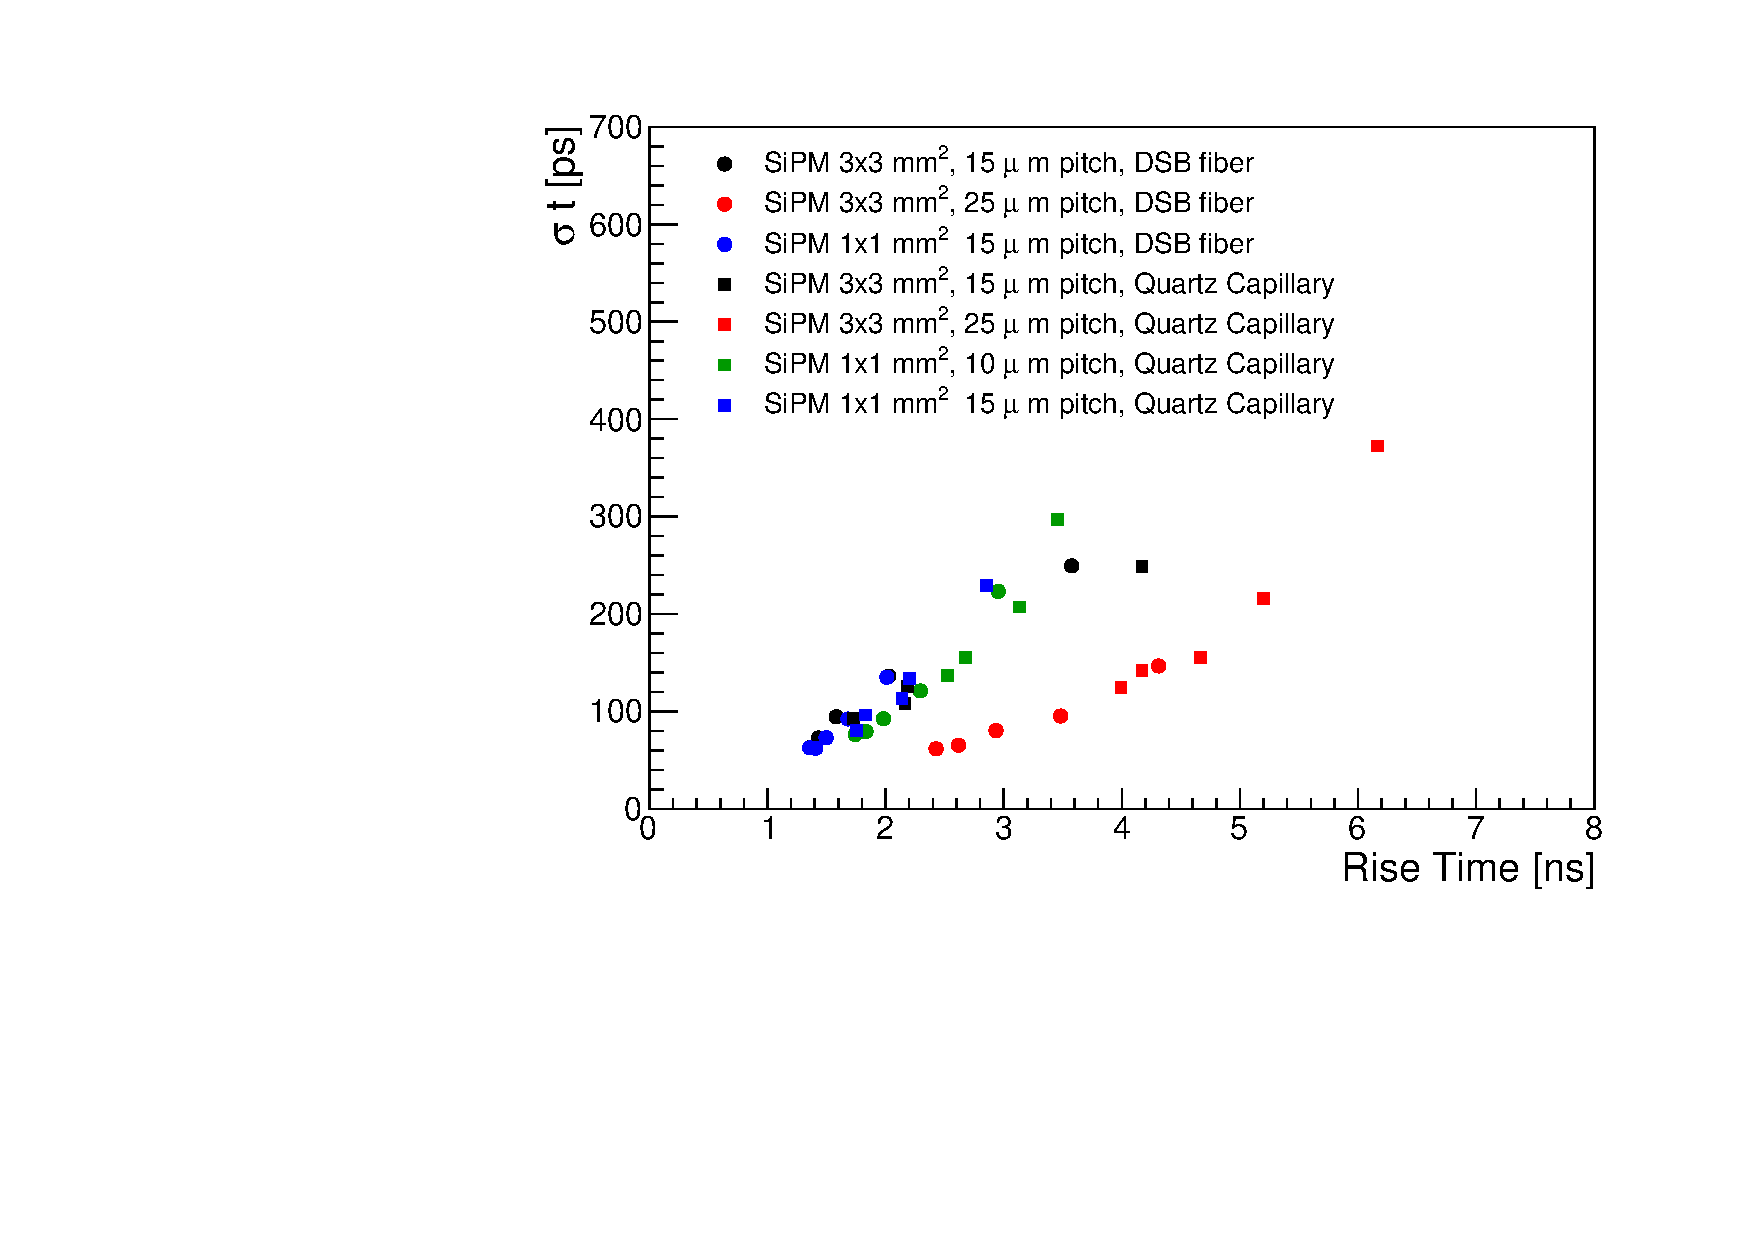
\includegraphics[width=0.48\textwidth]{figures/ShashlikTimeResolutionVsRiseTime.pdf}
\includegraphics[width=0.51\textwidth]{figures/ShashlikRiseTimeVsAmplitude.pdf}
\caption{\label{RiseTime}Time resolution is measured as a function of the rise time
for the four different SiPMs. The data recorded with the DSB WLS fibers and the
quartz capillaries are distinguished as dots and squares, respectively. }
\end{figure}

In our previous study~\cite{Anderson:2015gha} that used MCPs as photodetectors,
the rise time was measured to be about $3.0$~ns and did not have any dependence
on the signal amplitude. The very fast rise time of less than 150 ps of the MCP
and its signal amplitude linearity implied that the rise time was dominated by
the time constant of the wavelength shifter. In contrast, for the data presented
here using SiPMs as photodetectors, we observe that the rise time varies between
$1.4$~ns and $6$~ns. We attribute this effect to the fact that
there are so many scintillation photons reaching the SiPM that the signal is in
the non-linear saturation regime of the SiPM. As a result the signal appears to reach
its maximum faster. This effect is reproduced by a simple simulation where we 
take a scintillation light pulse with a rise time of $3$~ns impinging upon a
$1\times1$~$\mathrm{mm}^{2}$ SiPM with $10$~$\mu$m pixel size and 
simulate a dead time that is much larger than the rise time, on the order of
a few tens to a hundred nanoseconds.

of $5$~ns for each pixel. The resulting rise time as a function
of light input is shown in Figure~\ref{RiseTimeSimulation}, and shows a 
decreasing rise time as the amount of light increases.

\begin{figure}[!htb]
\centering
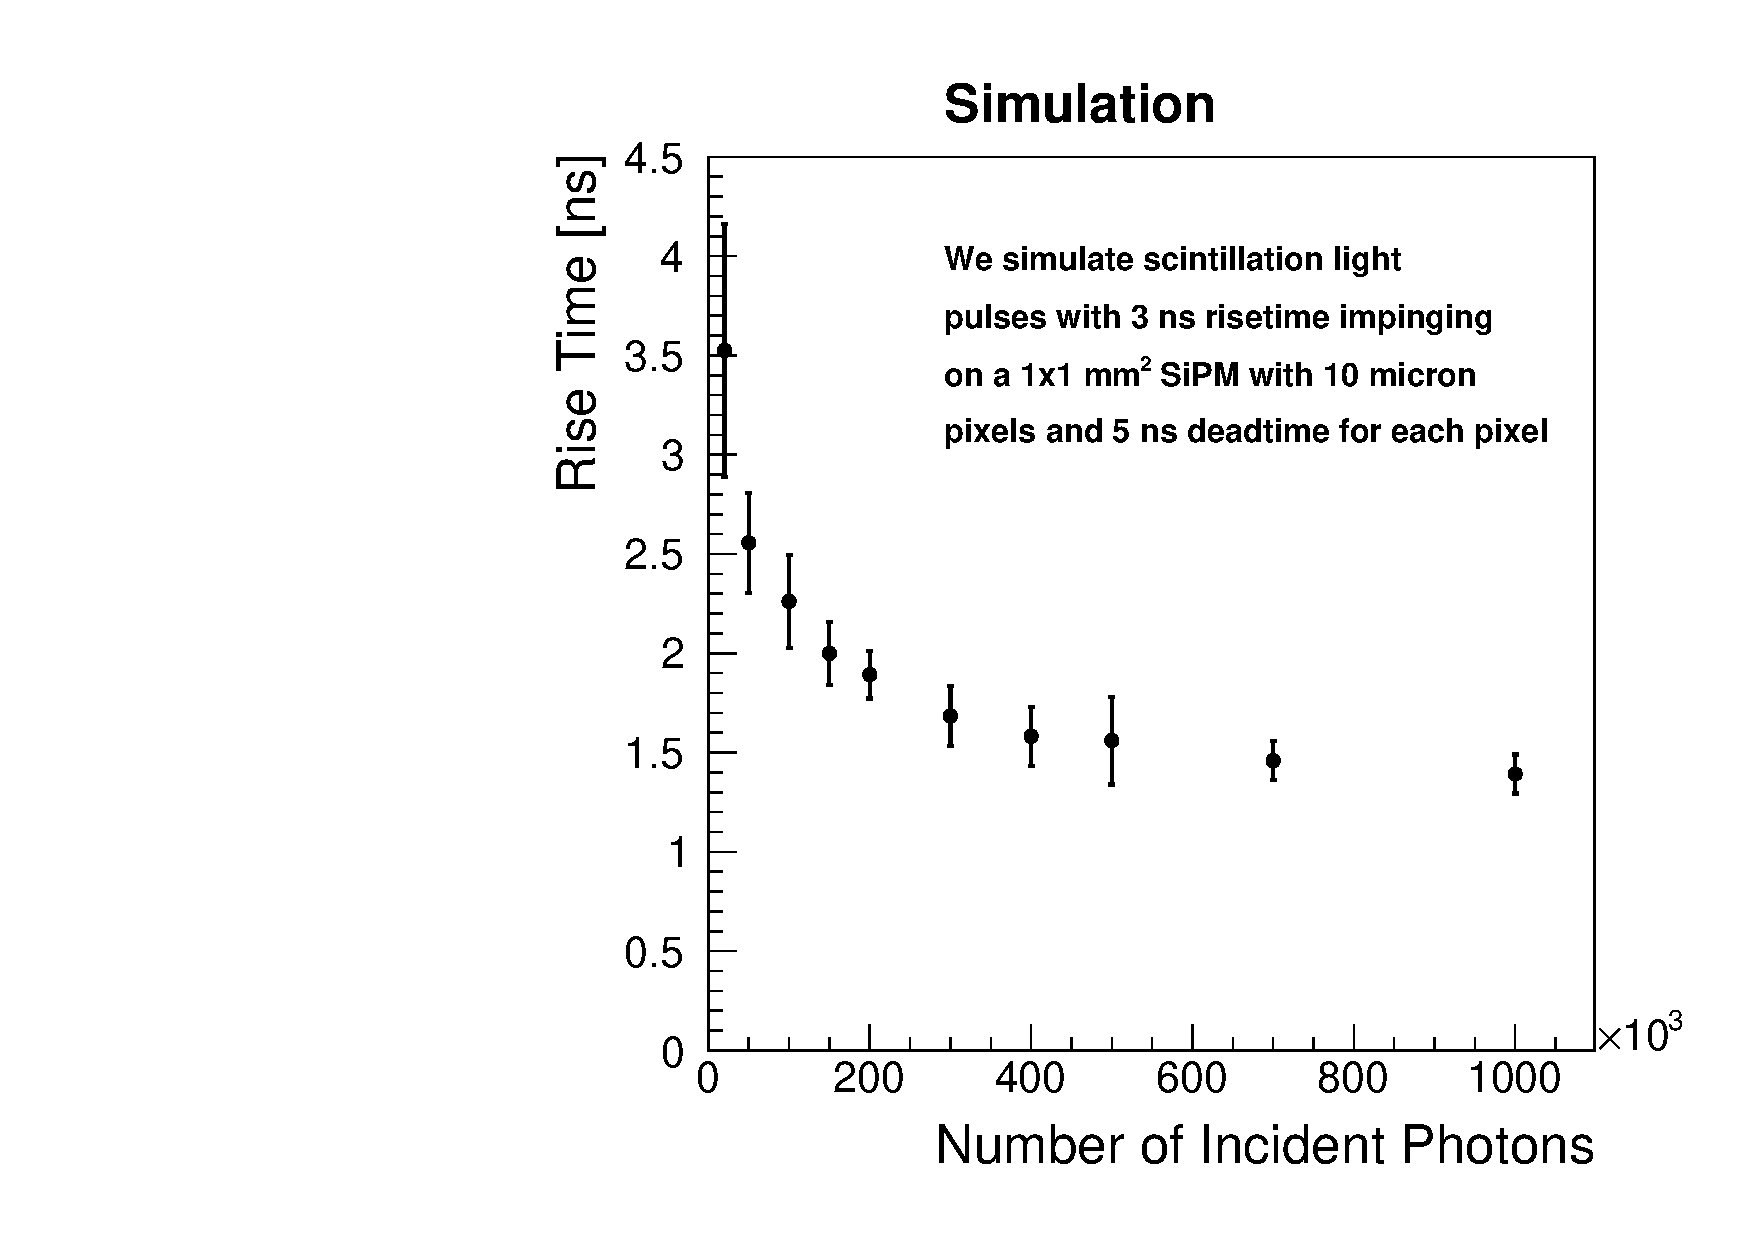
\includegraphics[width=0.99\textwidth]{figures/RisetimeSimulation.pdf}
\caption{\label{RiseTimeSimulation} We simulate a scintillation light pulse 
with a rise time of $3$~ns impinging upon a $1\times1$~$\mathrm{mm}^{2}$ 
SiPM with $10$~$\mu$m pixel size where each pixel has a dead time 
of $5$~ns. The resulting rise time of the full signal pulse is plotted as a function
of the amount of input scintillation light.}
\end{figure}

We show the time resolution measured as a function of the beam energy for
signals read out by DSB-doped WLS fibers and quartz capillaries in
Figure~\ref{TimeResolutionVsEnergy}. Finally, by combining the measured
timestamp from all four SiPM channels, we can significantly improve the time
resolution. The combined time resolution measurements for the DSB WLS fibers and
the quartz capillaries are shown in Fig~\ref{TimeResolutionCombined} and
demonstrate that we can achieve time resolution of $42$~ps for high energy
electromagnetic showers. The timing performance we achieve with the SiPM readout
is slightly better than the performance achieved with an MCP-PMT as in our
previous publication~\cite{Anderson:2015gha}, where we achieved $90$, $70$, and
$60$~ps at $50$, $100$, and $150$~GeV  respectively. 


\begin{figure}[!htb]
\centering
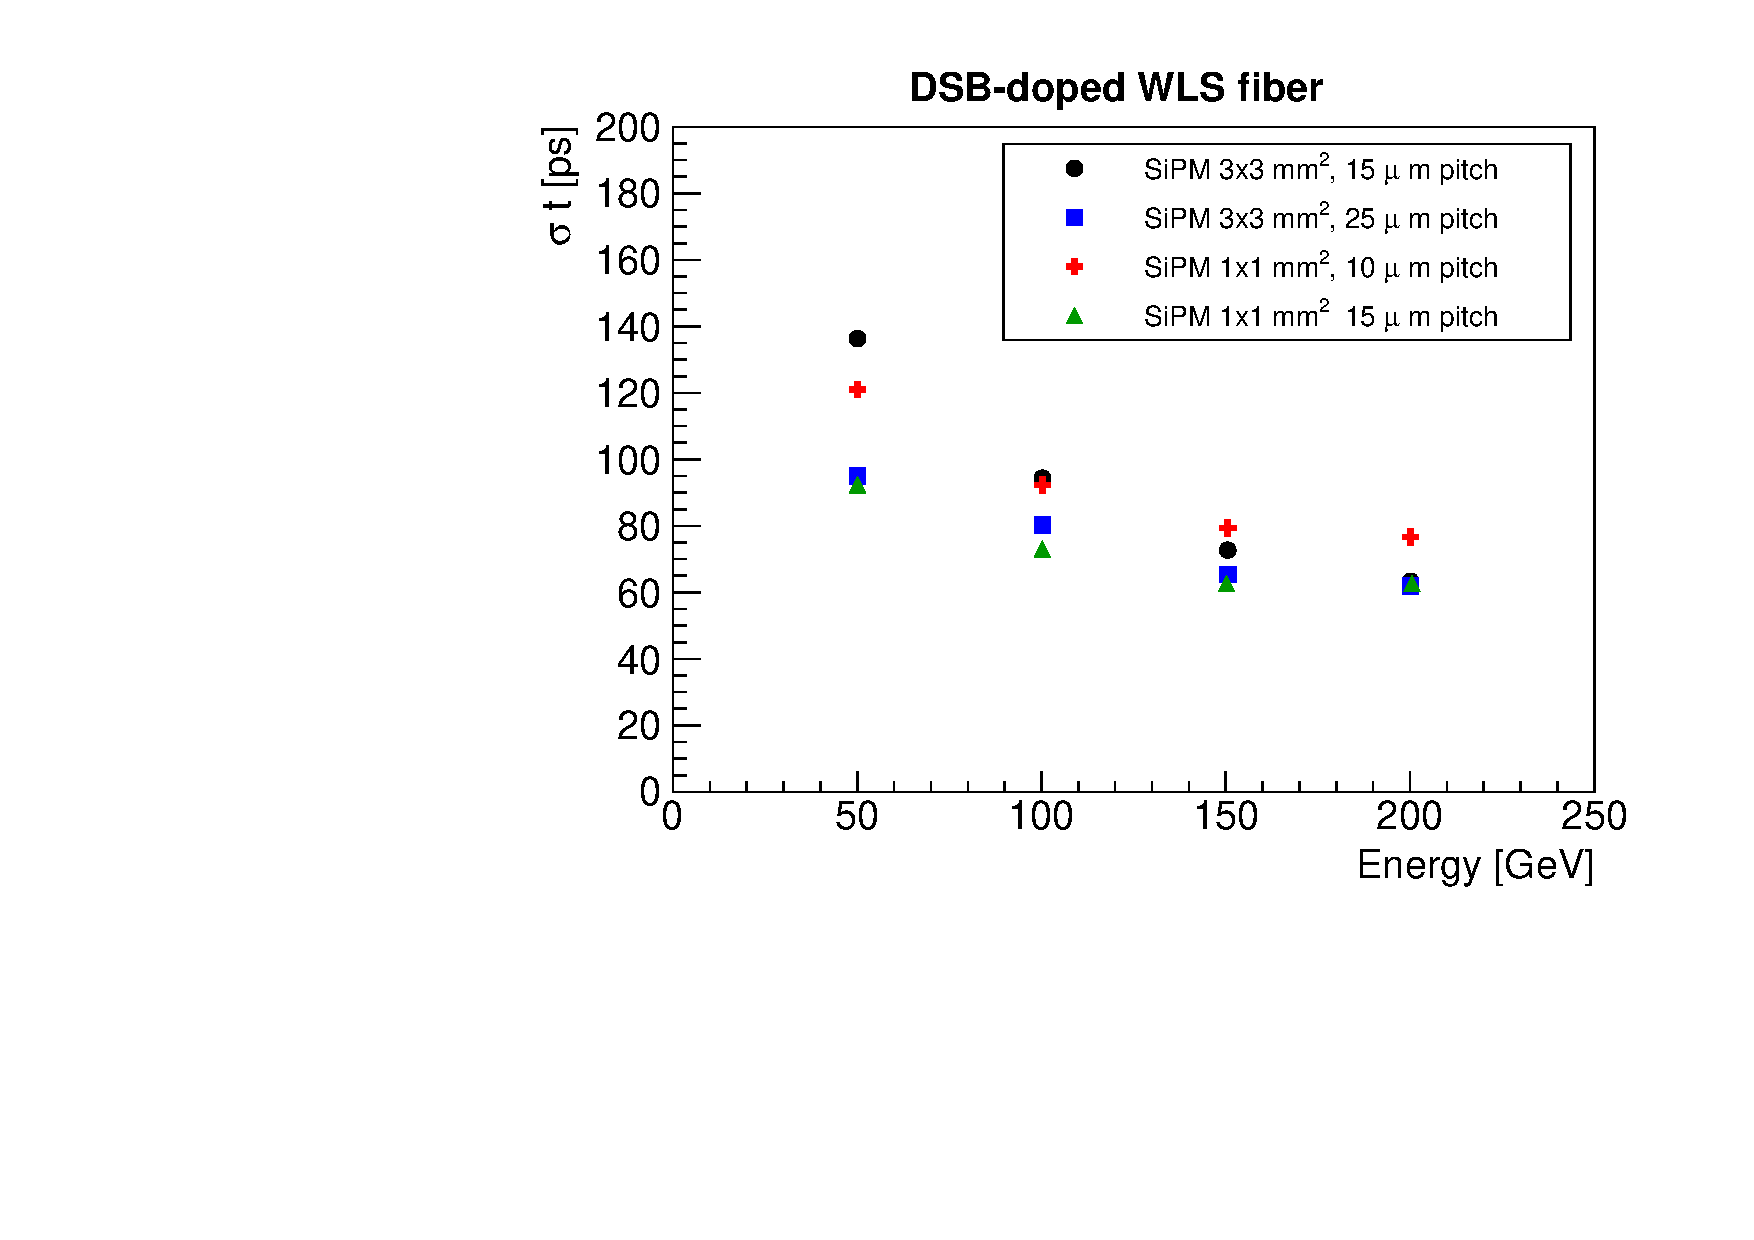
\includegraphics[width=0.49\textwidth]{figures/ShashlikTimeResolutionVsEnergy_DSB.pdf}
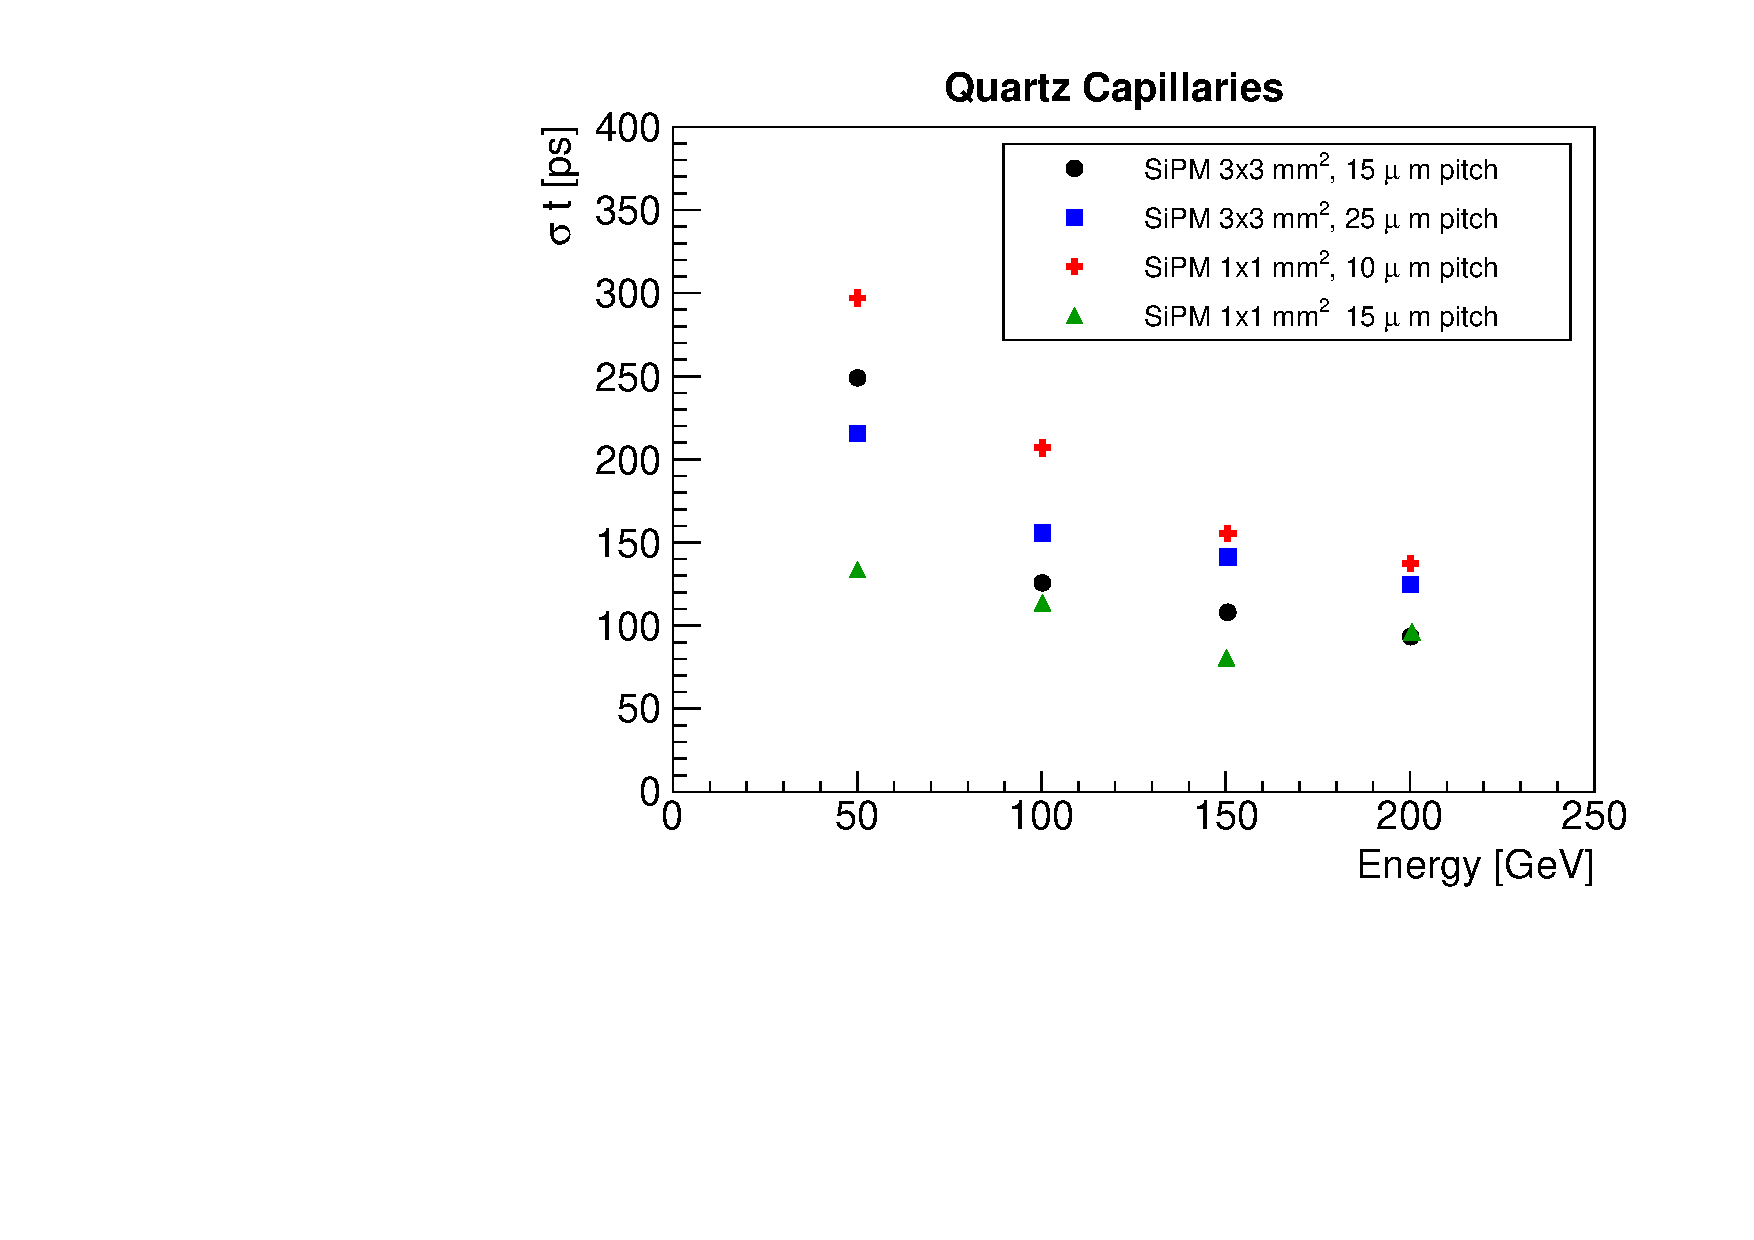
\includegraphics[width=0.49\textwidth]{figures/ShashlikTimeResolutionVsEnergy_Capillaries.pdf}
\caption{\label{TimeResolutionVsEnergy} Time resolution measured in the sampling calorimeter 
cell using the signal of each of the SiPMs individually as a function of the beam energy. 
The data taken using DSB-doped WLS fibers are shown on
the left and the data taken using DSB-filled quartz capillaries are shown on the right}
\end{figure}



\begin{figure}[!htb]
\centering
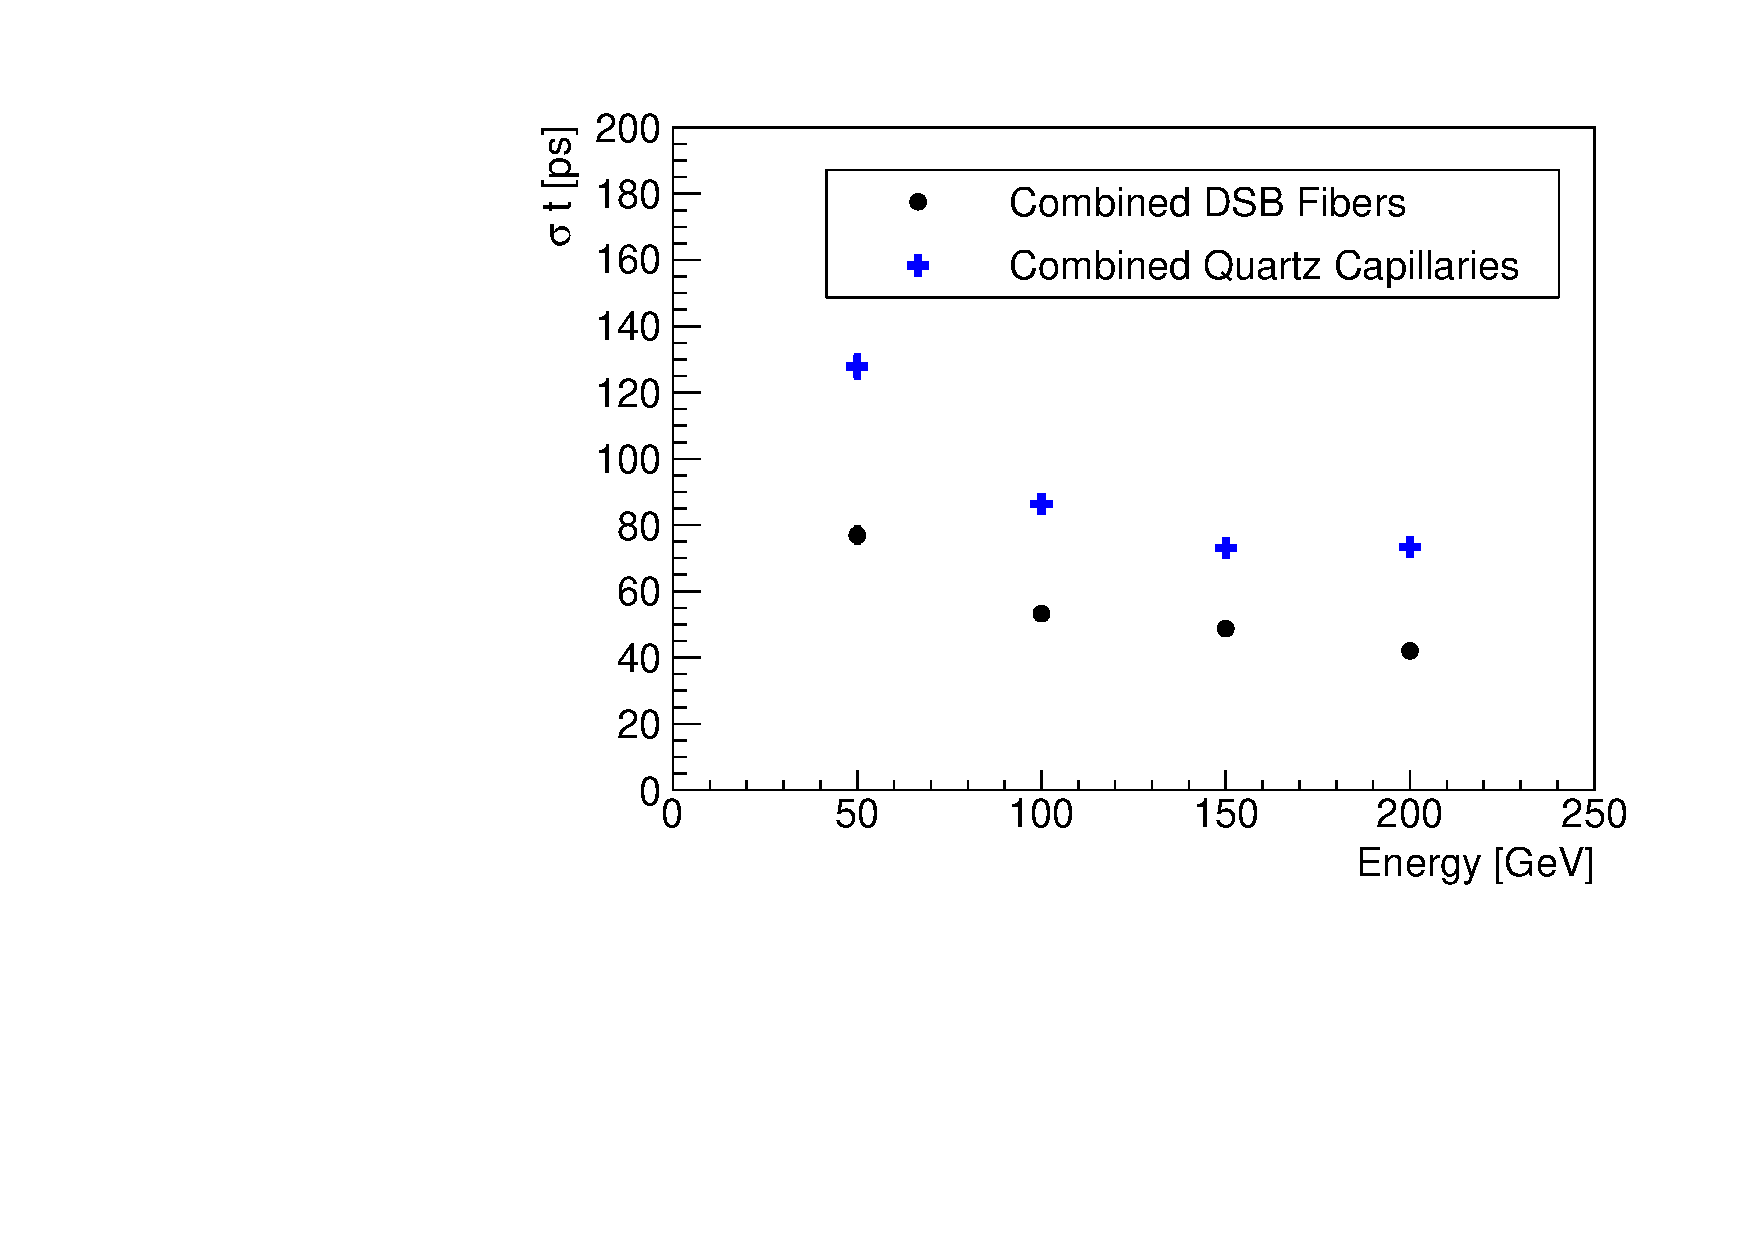
\includegraphics[width=0.8\textwidth]{figures/ShashlikTimeResolutionCombinedChannelVsEnergy.pdf}
\caption{\label{TimeResolutionCombined}  Time resolution measured in the sampling calorimeter cell combining signals from all four  
SiPMs is shown as a function of the beam energy.  The data recorded with the DSB-doped WLS fibers and the
DSB-filled quartz capillaries are distinguished as dots and squares.}
\end{figure}



The light extraction efficiency of capillaries with liquid WLS remains
sufficiently high for dose rates of $100$~Mrad and beyond and for fluences of
$10^{14}$~protons/$\mathrm{cm}^{2}$ and beyond~\cite{shashlik2}. This result
demonstrates the feasibility of achieving good time resolution using a sampling
calorimeter based on LYSO, which can survive in dense hadronic collision
environments. The timing performance could be further improved by increasing
the signal size, for example by using larger diameter capillaries or increasing
the calorimeter sampling fraction. 

